\documentclass{article}
\usepackage{tikz}
\usetikzlibrary{shapes}

\begin{document}

\textwidth=7in
\textheight=9.5in
\topmargin=-1in
\headheight=0in
\pagestyle{empty}

\begin{center}
{\bf CS 165 - Database Systems \\
 Homework 8 - Indexing \\
 Submission: March 8, 2014 (class)}
\end{center}

\vskip.35in
\noindent Given a B-tree index:

\begin{center}
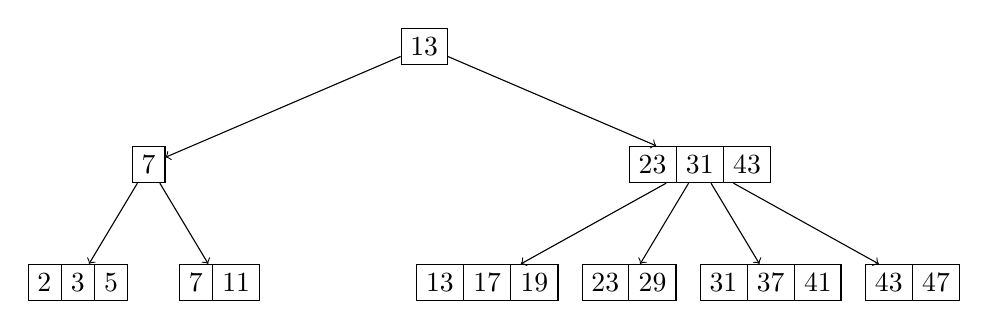
\begin{tikzpicture}
\tikzstyle{bplus}=[
	rectangle split,
	rectangle split horizontal,
	rectangle split ignore empty parts,
	draw ]
\tikzstyle{every node}=[bplus]
\tikzstyle{level 1}=[sibling distance=70mm]
\tikzstyle{level 2}=[sibling distance=18mm]
\node {13} [->]
	child {node {7}
    child {node {2 \nodepart{two} 3 \nodepart{three} 5}}
    child {node {7 \nodepart{two} 11}}
  }
  	child {node {23 \nodepart{two} 31 \nodepart{three} 43}
  	child {node {13 \nodepart{two} 17 \nodepart{three} 19}}
  	child {node {23 \nodepart{two} 29}}
  	child {node {31 \nodepart{two} 37 \nodepart{three} 41}}
  	child {node {43 \nodepart{two} 47}}
  }
;
\end{tikzpicture}
\end{center}

\begin{itemize}
\item 1. [2 points] Draw the B-tree after inserting {\bf 15}.
\item 2. [2 points] Draw the B-tree after inserting {\bf 25}.
\item 3. [2 points] Draw the B-tree after deleting {\bf 13}.
\item 4. [2 points] Draw the B-tree after deleting {\bf 11}.
\item 5. [2 points] Draw the B-tree after deleting {\bf 7}.
\end{itemize}


\end{document}